\documentclass{math}

\usepackage{tikz}
\usetikzlibrary{math}

\title{Differential Equations}
\author{Alvin Lin}
\date{January 2018 - May 2018}

\begin{document}

\maketitle

\section*{Concept Review}
\begin{align*}
  \int\frac{\diff{x}}{1+x^2} &\ne \ln(1+x^2)+c \\
  \int\frac{\diff{x}}{1+x^2} &= \arctan(x)+c
\end{align*}

\subsubsection*{Example}
\begin{align*}
  \int\frac{x}{1+x^2}\diff{x} \\
  Let: u &= x^2+1 \\
  \diff{u} &= 2x\diff{x} \\
  \frac{\diff{u}}{2} = x\diff{x} \\
  \int\frac{x}{1+x^2}\diff{x} &= \frac{1}{2}\int\frac{\diff{u}}{u} \\
  &= \frac{1}{2}\ln|u|+c \\
  &= \frac{1}{2}\ln|x^2+1|+c
\end{align*}

\subsubsection*{Example}
\begin{align*}
  \int\e^{2x}\diff{x} &\ne \frac{\e^{2x+1}}{2x+1}+c \\
  &= \frac{1}{2}\e^{2x}+c
\end{align*}

\subsubsection*{Example}
\begin{align*}
  \int\ln(x)\diff{x} \\
  Let: u &= \ln(x) \quad \diff{v} = \diff{x} \\
  \diff{u} &= \diff{x} \quad v = x \\
  &= x\ln(x)-\int{x\diff{x}}
\end{align*}

\subsubsection*{Properties of Logs}
\begin{enumerate}
  \item \( \ln(ab) = \ln(a)+\ln(b) \) given \( a,b\ne0 \)
  \item \( \ln(\frac{a}{b}) = \ln(a)-\ln(b) \)
  \item \( r\ln(a) = \ln(a^r) \)
\end{enumerate}

\subsubsection*{Rules of Exponents}
\begin{enumerate}
  \item \( \e^{x+y} = \e^x\e^y \)
  \item \( \e^{x-y} = \frac{\e^x}{\e^y} \)
  \item \( \e^{x^y} = \e^{xy} \)
\end{enumerate}

\section*{Solutions and Initial Value Problems}
A differential equation is an equation that contains one or more derivatives of
some unknown function.
\[ y''-\frac{2}{x^2}y = 0 \]
Using Leibniz's Notation:
\[ \ddiff{^2y}{x^2}-\frac{2}{x^2}y(x) = 0 \]
Another example:
\[ y''+3y'+2y = 0 \]
A function \( \phi \) defined on some interval \( I \) having at least \( n \)
continuous derivatives on \( I \), is an explicit solution over \( I \) if it
satisfies the equation on \( I \).

\subsection*{Classification by Order and Linearity}
The order of a differential equation is the order of the highest derivative that
appears in the equation.
\[ y'''+2y'+y = \e^x \]
is a third order equation. With respect to linearity, consider the following:
\[ a_n(x)y^{(n)}+a_{n-1}y^{(n-1)}+\dots+a_1(x)y'+a_0(x)y = g(x) \]
where \( a_n(x) \) is a function of the independent variable only,
\( y^{(n)} \) is a derivative to the n\textsuperscript{th} power and \( g(x) \)
is a function of \( x \) only.
\begin{itemize}
  \item \( \ddiff{^2y}{x^2} = -\cos(y) \) is a non-linear, second-order
  differential equation.
  \item \( y''+\ln(y)y'-5y = \e^x \) is a non-linear, second-order differential
  equation.
  \item \( y''+\ln(x)y-5y = \e^x \) is a linear, second-order differential
  equation.
\end{itemize}

\subsubsection*{Example}
Show that \( y = \phi(x) = x^2-\frac{1}{x} \) is an explicit solution to
\( y''-\frac{2}{x^2}y = 0 \).
\begin{align*}
  y &= x^2-\frac{1}{x} \\
  y' &= 2x+x^{-2} \\
  y'' &= 2-2x^{-3} \\
  y''-2\frac{x^2}y &= 2-2x^{-3}-\frac{2}{x^2}(x^2-\frac{1}{x}) \\
  &= 2-\frac{2}{x^3}-2+\frac{2}{x^3} \\
  &= 0
\end{align*}
Hence, \( y \) satisfies this differential equation.

\subsubsection*{Example}
Verify that \( y(t)=\e^{-2t}\sin(4t) \) is a solution to \( y''+4y'+20y = 0 \).
\begin{align*}
  y &= \e^{-2t}\sin(4t) \\
  y' &= -2\e^{-2t}\sin(4t)+\e^{-2t}(4)\cos(4t) \\
  y'' &= 4\e^{-2t}\sin(4t)+(-2\e^{-2t})(4)\cos(4t)+(4)(-2\e^{-2t})\cos(4t)+
    \e^{-2t}(-16)\sin(4t) \\
  y''+4y'+20y &= 4\e^{-2t}\sin(4t)-8\e^{-2t}\cos(4t)-8\e^{-2t}\cos(4t)- \\
    &~~~~ 16\e^{-2t}\sin(4t)+
      4\bigg(-2\e^{-2t}\sin(4t)+4\e^{-2t}\cos(4t)\bigg)+ \\
    &~~~~ 20\e^{-2t}\sin(4t) \\
  &= 24\e^{-2t}\sin(4t)-24\e^{-2t}\sin(4t)+
    16\e^{-2t}\cos(4t)-16\e^{-2t}\cos(4t) \\
  &= 0
\end{align*}

\subsubsection*{Example}
Verify that \( y = c_1\e^t+c_2\e^{2t} \) is an explicit solution to
\( y''-3y'+2y = 0 \) for any constants \( c_1 \) and \( c_2 \).
\begin{align*}
  y &= c_1\e^t+c_2\e^{2t} \\
  y' &= c_1\e^t+2c_2\e^{2t} \\
  y'' &= c_1\e^t+4c_2\e^{2t} \\
  y''-3y'+2y &= c_1\e^t+4c_2\e^{2t}-
    3\bigg(c_1\e^t+2c_2\e^{2t}\bigg)+2\bigg(c_1\e^t+c_2\e^{2t}\bigg) \\
  &= 0
\end{align*}

\subsection*{Implicit Solutions}
A relation \( G(x,y) = 0 \), is an \textbf{implicit} solution if it determines
one or more explicit solutions. For example, verify that \( x^2-\sin(x+y) = 1 \)
is an implicit solution to \( \ddiff{y}{x} = 2x\sec(x+y)-1 \). Differentiating
\( x^2-\sin(x+y) = 1 \) implicitly, we get:
\begin{align*}
  2x-\cos(x+y)\ddiff{}{x}(x+y) &= 0 \\
  2x-\cos(x+y)(1+\ddiff{y}{x}) &= 0 \\
  2x-\cos(x+y)-\cos(x+y)\ddiff{y}{x} &= 0 \\
  2x-\cos(x+y) &= \cos(x+y)\ddiff{y}{x} \\
  \ddiff{y}{x} &= \frac{2x}{\cos(x+y)}-1 \\
  &= 2x\sec(x+y)-1
\end{align*}

\subsubsection*{Example}
Show \( x+y+\e^{xy} = 0 \) is an implicit solution to \( (1+x\e^{xy})
\ddiff{y}{x}+1+y\e^{xy} = 0 \).
\begin{align*}
  x+y+\e^{xy} &= 0 \\
  1+\ddiff{y}{x}+\e^{xy}\bigg[\ddiff{}{x}(xy)\bigg] &= 0 \\
  1+\ddiff{y}{x}+\e^{xy}\bigg[y+x\ddiff{y}{x}\bigg] &= 0 \\
  1+\ddiff{y}{x}+y\e^{xy}+x\e^{xy}\ddiff{y}{x} &= 0 \\
  1+\bigg[1+x\e^{xy}\bigg]\ddiff{y}{x}+y\e^{xy} &= 0 \\
  (1+x\e^{xy})\ddiff{y}{x}+1+y\e^{xy} &= 0
\end{align*}

\subsubsection*{Example}
Show that \( x^2+y^2-25 = 0 \) is an implicit solution to \( \ddiff{y}{x} =
f(x,y) = \frac{-x}{y} \) on \( (-5,5) \).
\begin{align*}
  x^2+y^2-25 &= 0 \\
  2x+2y\ddiff{y}{x} &= 0 \\
  y\ddiff{y}{x} &= -x \\
  \ddiff{y}{x} &= \frac{-x}{y}
\end{align*}
Alternatively, we can try doing this explicitly by solving for \( y \):
\begin{align*}
  y^2 &= 25-x^2 \\
  y &= \pm\sqrt{25-x^2} \\
  \text{Choose } y &= \sqrt{25-x^2} \\
  &= (25-x^2)^{\frac{1}{2}} \\
  y' &= \frac{1}{2}\left(25-x^2\right)^{-\frac{1}{2}}(-2x) \\
  &= \frac{-x}{\sqrt{25-x^2}} \\
  &= \frac{-x}{y}
\end{align*}
We want to find where \( 25-x^2 > 0 \), which tells us that \( -5 < x < 5 \).

\subsection*{Families of Solutions}
Let's try to solve the following:
\begin{align*}
  \ddiff{y}{x} &= \frac{-y}{x} = f(x,y) \\
  &= (-y)\frac{1}{x} \\
  \frac{\diff{y}}{y} &= -\frac{\diff{x}}{x} \\
  \int\frac{\diff{y}}{y} &= -\int\frac{\diff{x}}{x} \\
  \ln|y| &= -\ln|x|+c
\end{align*}
This is an \textbf{implicit} solution to our differential equation. We can also
try to solve it explicitly by exponentiating both sides.
\begin{align*}
  \ln|y| &= -\ln|x|+c \\
  \e^{\ln|y|} &= \e^{(-\ln|x|+c)} \\
  |y| &= \e^{-\ln|x|}\e^c \\
  |y| &= \e^{\ln|x^{-1}|}\e^c \\
  &= \left|\frac{1}{x}\right|\e^c
\end{align*}
If we let \( k = \pm\e^c \), then:
\begin{align*}
  y &= \pm\frac{1}{x}\e^c \\
  &= \frac{k}{x}
\end{align*}
This is a \textbf{family} of one parameter \( k \) solutions. It is a general
solution that contains an arbitrary constant \( k \). Suppose we are given an
initial value \( y(1) = 5 \), which lies on one of the curves.
\[ y = \frac{k}{x} \Longrightarrow 5 = \frac{k}{1} \Longrightarrow k = 5 \]
\( y = \frac{5}{x} \) is a \textbf{particular} solution since there are no
arbitrary constants.

\subsection*{n\textsuperscript{th} Order Initial Value Problems}
Given \( F(x,y,y',y'',\dots,y^{(n)}) = 0 \) and \( n \) initial conditions:
\begin{align*}
  y(x_{\circ}) &= y_0 \\
  y'(x_{\circ}) &= y_1 \\
  y''(x_{\circ}) &= y_2 \\
  & \vdots \\
  y^{(n-1)}(x_{\circ}) &= y_{n-1}
\end{align*}
We have an initial value problem. The solution over some interval \( I \) is
called a particular solution.

\subsubsection*{Example}
Verify that \( y = c_1\cos(x)+c_2\sin(x)-\sin(2x) \) is a general solution to
\( y''+y = 3\sin(2x) \).
\begin{align*}
  y &= c_1\cos(x)+c_2\sin(x)-\sin(2x) \\
  y' &= -c_1\sin(x)+c_2\cos(x)-2\cos(2x) \\
  y'' &= -c_1\cos(x)-c_2\sin(x)+4\sin(2x) \\
  y''+y &= 3\sin(2x)
\end{align*}
\begin{align*}
  -c_1\cos(x)-c_2\sin(x)+4\sin(2x)+c_1\cos(x)+c_2\sin(x)-\sin(2x) &=
    3\sin(2x) \\
  3\sin(2x) &= 3\sin(2x)
\end{align*}
Find constants \( c_1 \) and \( c_2 \) so that the initial conditions
\( y(0) = 1 \) and \( y'(0) = 0 \) are satisfied.
\begin{align*}
  y &= c_1\cos(x)+c_2\sin(x)-\sin(2x) \\
  y(0) &= 1 = c_1\cos(0) \\
  c_1 &= 1 \\
  y' &= -c_1\sin(x)+c_2\cos(x)-2\cos(2x) \\
  y'(0) &= 0 = 0+c_2-2 \\
  c_2 &= 2 \\
  y &= \cos(x)+2\sin(x)-\sin(2x)
\end{align*}

\subsubsection*{Example}
Determine whether \( y = c_1\e^{2t}+c_2t\e^{2t} \) is a general solution to
\( y''-4y'+4y = 0 \).
\begin{align*}
  y &= c_1\e^{2t}+c_2t\e^{2t} \\
  y' &= 2c_1\e^{2t}+c_2\e^{2t}+2c_2t\e^{2t} \\
  y'' &= 4c_1\e^{2t}+2c_2\e^{2t}+2c_2\e^{2t}+4c_2t\e^{2t} \\
  y''+4y'+2y &= 4c_1\e^{2t}+2c_2\e^{2t}+2c_2\e^{2t}+4c_2t\e^{2t}- \\
    &~~~~ 4\left(2c_1\e^{2t}+c_2\e^{2t}+2c_2t\e^{2t}\right)+ \\
    &~~~~ 4\left(c_1\e^{2t}+c_2t\e^{2t}\right) \\
  &= 0
\end{align*}
Find constants \( c_1 \) and \( c_2 \) such that the initial conditions
\( y(0) = 1 \) and \( y'(0) = 0 \) are satisfied.
\begin{align*}
  y(0) &= 1 = c_1 \\
  y'(0) &= 1 = 2+c_2 \\
  c_2 &= -1
\end{align*}

\subsection*{Direction Fields of 1st Order Equations}
Consider the following:
\[ \ddiff{y}{x} = f(x,y) \]
\( x \) is the independent variable and \( y \) is the dependent variable.
\begin{center}
  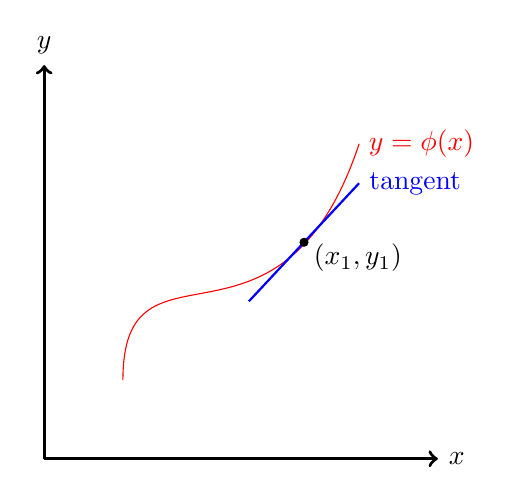
\begin{tikzpicture}
    \draw[very thick,->] (0,0) -- (5,0) node[right] {\( x \)};
    \draw[very thick,->] (0,0) -- (0,5) node[above] {\( y \)};
    \draw[red] (1,1) .. controls (1,3) and (3,1) .. (4,4)
      node[right] {\( y = \phi(x) \)};
    \draw[thick, blue] (2.6,2) -- (4,3.5) node[right] {tangent};
    \draw[fill] (3.3,2.75) circle (0.05cm)
      node[right,yshift=-0.2cm] {\( (x_1,y_1) \)};
  \end{tikzpicture}
\end{center}
The idea is that the actual solution curve is \( y = \phi(x) \). If we
evaluate \( \ddiff{y}{x} = f(x_1,y_1) \), it gives the slope of the
tangent at \( (x_1, y_1) \). We can construct a direction field with this. For
example, if we have the differential equation \( \ddiff{y}{x} = \frac{-y}{x} \).
\begin{minipage}[c]{8cm}
  \begin{center}
    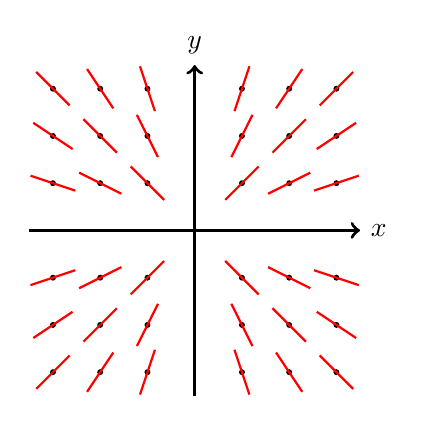
\begin{tikzpicture}[scale=0.6]
      \draw[very thick,->] (-3.5,0) -- (3.5,0) node[right] {\( x \)};
      \draw[very thick,->] (0,-3.5) -- (0,3.5) node[above] {\( y \)};
      \foreach \x in {-3,-2,-1,1,2,3} {
        \foreach \y in {-3,-2,-1,1,2,3} {
          \tikzmath{
            \m = \y/\x;
            \ang = atan(\m);
            \xa = \x-(0.5*cos(\ang));
            \ya = \y-(0.5*sin(\ang));
            \xb = \x+(0.5*cos(\ang));
            \yb = \y+(0.5*sin(\ang));
          };
          \draw[fill] (\x,\y) circle (0.05cm);
          \draw[thick,red] (\xa,\ya) -- (\xb,\yb);
        }
      }
    \end{tikzpicture}
  \end{center}
\end{minipage}
\begin{minipage}[c]{8cm}
  \begin{tabular}{|c|c|c|}
    \hline
    \( x \) & \( y \) & \( \ddiff{y}{x} \) \\
    \hline
    1 & 1 & -1 \\
    \hline
    1 & 2 & -2 \\
    \hline
    1 & 3 & -3 \\
    \hline
    1 & -1 & 1 \\
    \hline
    -1 & 1 & 1 \\
    \hline
  \end{tabular}
\end{minipage}

\subsection*{Autonomous First-Order Equations}
Autonomous first-order equations are equations of the form
\[ \ddiff{y}{x} = f(y) \]
where the independent variable \( x \) does not appear in the equation.
Consider the following:
\[ f(y) = \ddiff{y}{x} = y-y^2 \]
This is an autonomous equation. In contrast:
\[ \ddiff{y}{x} = xy = f(x,y) \]
This is not an autonomous equation. Equilibrium solutions are found by solving
\( f(y) = 0 = \ddiff{y}{x} \).
\begin{itemize}
  \item If \( y \) is bounded by a critical point, then the graph of \( y \)
  approaches \( y(t) = c \) as \( t\to+\infty \).
  \item \( \ddiff{y}{t} \) is either positive or negative except where
  \( \ddiff{y}{t} = 0 \).
  \item \( y \) is monotonic, either increasing or decreasing, there is no
  oscillation.
  \item The graph of non-constant soultions never cross an equilibrium solution.
\end{itemize}

\subsubsection*{Example}
A model for the velocity \( v \) at time \( t \) of an object falling under the
influence of gravity in a viscous medium is given by
\[ \ddiff{v}{t} = 1-\frac{v^3}{8} \]
Construct a direction field and determine the ``terminal'' velocity. Find values
where \( 1-\frac{v^3}{8} = 0 \).
\begin{center}
  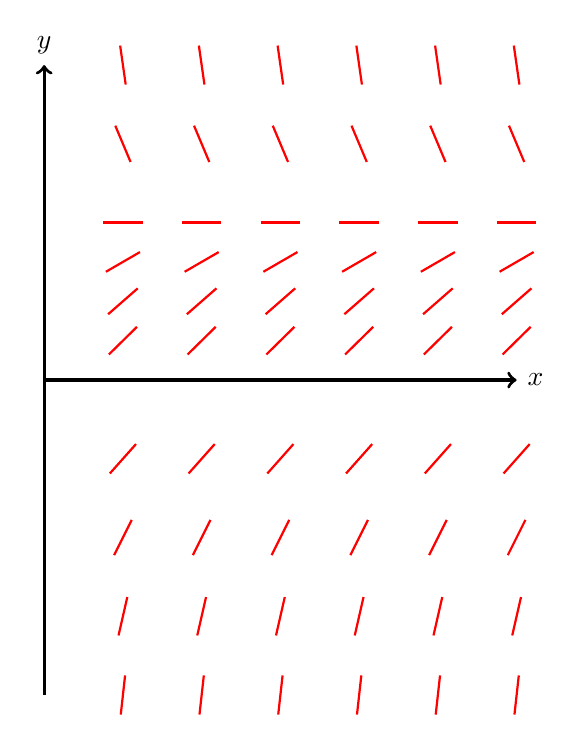
\begin{tikzpicture}
    \draw[very thick,->] (0,0) -- (6,0) node[right] {\( x \)};
    \draw[very thick,->] (0,-4) -- (0,4) node[above] {\( y \)};
    \foreach \t in {1,2,3,4,5,6} {
      \foreach \v in {-4,-3,-2,-1,0.5,1,1.5,2,3,4} {
        \tikzmath{
          \m = 1-((\v*\v*\v)/8);
          \ang = atan(\m);
          \ta = \t-(0.25*cos(\ang));
          \va = \v-(0.25*sin(\ang));
          \tb = \t+(0.25*cos(\ang));
          \vb = \v+(0.25*sin(\ang));
        };
        \draw[thick,red] (\ta,\va) -- (\tb,\vb);
      }
    }
  \end{tikzpicture}
\end{center}
\[ 1-\frac{v^3}{8} = 0 \Rightarrow v = 2 \]
From this diagram, we can see all the families of solutions for this
differential equation, but they all converge to \( v = 2 \) as \( t\to\infty \).

\subsubsection*{Example}
Consider the following equation for a population (in thousands) of a certain
species (Logistic Equation).
\[ \ddiff{p}{t} = 9p-7p^2 = f(p) \]
\[ \ddiff{p}{t} = 9p-7p^2 = 0 \Rightarrow p(9-7p) = 0 \]
Our solutions are \( p = 0 \) or \( p = \frac{9}{7} \).
\begin{center}
  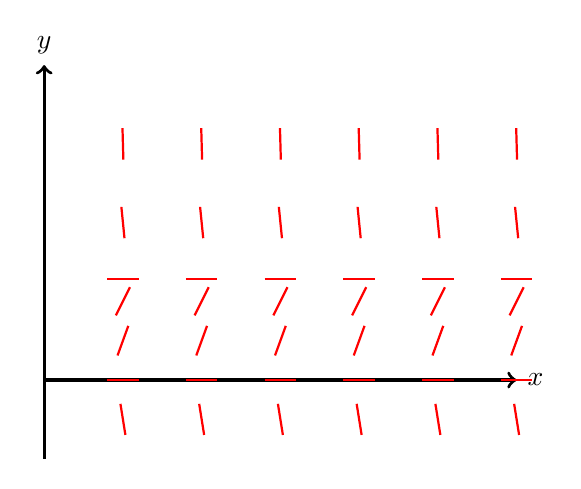
\begin{tikzpicture}
    \draw[very thick,->] (0,0) -- (6,0) node[right] {\( x \)};
    \draw[very thick,->] (0,-1) -- (0,4) node[above] {\( y \)};
    \foreach \t in {1,2,3,4,5,6} {
      \foreach \p in {-0.5,0,0.5,1,9/7,2,3} {
        \tikzmath{
          \m = (9*\p)-(7*\p*\p);
          \ang = atan(\m);
          \ta = \t-(0.2*cos(\ang));
          \pa = \p-(0.2*sin(\ang));
          \tb = \t+(0.2*cos(\ang));
          \pb = \p+(0.2*sin(\ang));
        };
        \draw[thick,red] (\ta,\pa) -- (\tb,\pb);
      }
    }
  \end{tikzpicture}
\end{center}
\[ \lim_{t\to\infty} = \frac{9}{7} \]

\subsection*{Euler's Method}
Euler's method is also known as the tangent line method for finding numerical
approximations to first-order initial value problems.
\begin{center}
  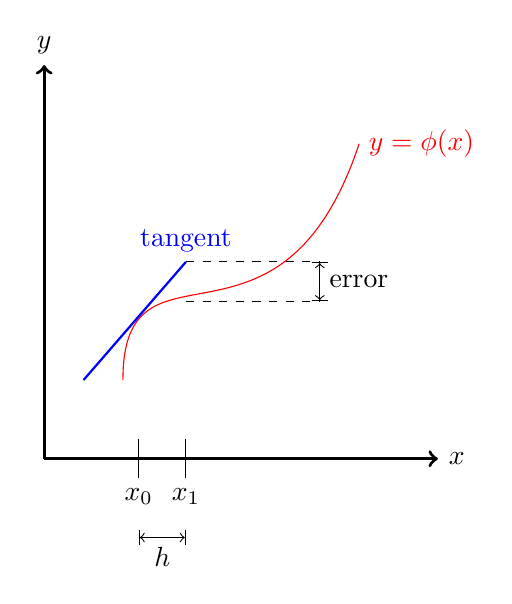
\begin{tikzpicture}
    \draw[very thick,->] (0,0) -- (5,0) node[right] {\( x \)};
    \draw[very thick,->] (0,0) -- (0,5) node[above] {\( y \)};
    \draw[red] (1,1) .. controls (1,3) and (3,1) .. (4,4)
      node[right] {\( y = \phi(x) \)};
    \draw[thick, blue] (0.5,1) -- (1.8,2.5) node[above] {tangent};
    \draw (1.2,0.25) -- (1.2,-0.25) node[below] {\( x_0 \)};
    \draw (1.8,0.25) -- (1.8,-0.25) node[below] {\( x_1 \)};
    \draw[|<->|] (1.2,-1) -- (1.8,-1) node[pos=0.5,below] {\( h \)};
    \draw[dashed] (1.8,2) -- (3.5,2);
    \draw[dashed] (1.8,2.5) -- (3.5,2.5);
    \draw[|<->|] (3.5,2) -- (3.5,2.5) node[pos=0.5,right] {error};
  \end{tikzpicture}
\end{center}
With this method, we also begin with some solution curve \( y = \phi(x) \) and
some given \( (x_0,y_0) \) that lies on the solution curve.
\begin{align*}
  \ddiff{y}{x} &= f(x,y) \\
  y(x_0) &= y_0
\end{align*}
\( f(x_0,y_0) \) is the slope of the tangent to the curve at \( (x_0,y_0) \).
Given \( (x_0,y_0) \), a single step \( h \), and the slope \( f(x_0,y_0) \):
\[ y-y_0 = h\big[f(x_0,y_0)\big] \]
\[ y_1 = y_0+h\big[f(x_0,y_0)\big] \]
This is an iterative process defined by:
\[ y_{n+1} = y_n+h\big[f(x_n,y_n)\big] \]
We determine the step size and iterate:
\begin{center}
  \begin{tabular}{|c|c|}
    \hline
    \( x_0 \) & \( y_0 \) \\
    \hline
    \( x_1 = x_0+h \) & \( y_1 \) \\
    \hline
    \( x_2 = x_1+h \) & \( y_2 \) \\
    \hline
    \vdots & \vdots \\
    \hline
    \( x_{n+1} = x_n+h \) & \( y_{n+1} \) \\
    \hline
  \end{tabular}
\end{center}

\subsubsection*{Example}
\[ \ddiff{y}{x} = x^2+y^2 = f(x,y) \]
If we take \( y(1) = 1 \) with \( h = 0.1 \) as our step size:
\begin{center}
  \begin{tabular}{|c|c|}
    \hline
    \( x_0 = 1 \) & \( y_0 = 1 \) \\
    \hline
    \( x_1 = 1.1 \) & \( y_1 = 1+0.1(2) = 1.2 \) \\
    \hline
    \\[-1em]
    \( x_2 = 1.2 \) & \( y_2 = 1.2+0.1[(1.1)^2+(1.2)^2] = 1.465 \) \\
    \hline
    \vdots & \vdots \\
    \hline
  \end{tabular}
\end{center}

\begin{center}
  You can find all my notes at \url{http://omgimanerd.tech/notes}. If you have
  any questions, comments, or concerns, please contact me at
  alvin@omgimanerd.tech
\end{center}

\end{document}
